%
% Copyright 2017 Markus Borg, Lund University
%
% This work is licensed under a Creative Commons Attribution-ShareAlike 4.0 International License.
% See http://creativecommons.org/licenses/by-sa/4.0/
%
% The dodument is based on a LaTeX template developed by Jean-Philippe Eisenbarth
% https://github.com/jpeisenbarth/SRS-Tex
%
\documentclass{scrreprt}
\usepackage{graphicx}
\usepackage{listings}
\usepackage{underscore}
\usepackage[bookmarks=true]{hyperref}
\usepackage[utf8]{inputenc}
\usepackage[english]{babel}
\usepackage{eurosym}
\hypersetup{
    bookmarks=false,    % show bookmarks bar?
    pdftitle={Project Instructions for the LU Rumble},    % title
    pdfauthor={Markus Borg},                     % author
    pdfsubject={TeX and LaTeX},                        % subject of the document
    pdfkeywords={TeX, LaTeX, graphics, images}, % list of keywords
    colorlinks=true,       % false: boxed links; true: colored links
    linkcolor=blue,       % color of internal links
    citecolor=black,       % color of links to bibliography
    filecolor=black,        % color of file links
    urlcolor=purple,        % color of external links
    linktoc=page            % only page is linked
}%
\def\myversion{0.86 }
\date{}
%\title
\usepackage{hyperref}
\begin{document}

\begin{flushright}
    \rule{16cm}{5pt}\vskip1cm
    \begin{bfseries}
    	\LARGE{ETSA02-ADM-INS}\\
    	\vspace{1.5cm}
        \Huge{Project\\ Instructions}\\
        \vspace{0.5cm}
        for\\
        \vspace{0.5cm}
        the LU Rumble\\
        \vspace{1.5cm}
        \LARGE{Version \myversion}\\ %approved}\\
        \vspace{1.5cm}
        Prepared by Markus Borg\\
        %\vspace{1.5cm}
        Dept. of Computer Science, Lund University\\
        \vspace{1.5cm}
        \today\\
    \end{bfseries}
\end{flushright}

\tableofcontents


\chapter*{Revision History}

\begin{center}
    \begin{tabular}{|c|c|p{8cm}|c|}
        \hline
	    Name & Date & Change description & Version\\
        \hline
	    Markus Borg & 2017-12-07 & Initial draft. & 0.1\\
        \hline
        Markus Borg & 2017-12-27 & Complete draft of intro, engineering, monetizing, and strategizing. Sent for external review. & 0.2\\
        \hline
        Markus Borg & 2017-12-31 & First draft of sprints. & 0.3\\
        \hline
        Markus Borg & 2018-01-02 & First complete draft. & 0.4\\
        \hline
        Markus Borg & 2018-02-05 & Updated after internal review. & 0.5\\
        \hline
        Markus Borg & 2018-03-06 & Updated after external review. & 0.6\\
        \hline
        Markus Borg & 2018-03-08 & Minor consistency improvements. & 0.7\\
        \hline
        Markus Borg & 2018-03-24 & Updated after course start. Added robot communication, releases and deliverables. & 0.8\\
        \hline
        Markus Borg & 2018-03-29 & Replaced test specification with STS. Fixed L4 dates. Introduced RoboTalk. & 0.85\\
        \hline
        Markus Borg & 2018-04-18 & Clarified the discount rule for Robot Market & 0.86\\
        \hline
    \end{tabular}
\end{center}

\chapter{Introduction}
This document describes the project in ETSA02 Introduction to Software Engineering -- Methodology. Together with other students, you will work together to engineer a robot for competition in LU Rumble -- a local instance of team battles in Robocode, a programming game in which robots compete in battles without human intervention by executing their programs.

In the remainder of this document, we use the term ``group'' to refer to the students working together during the project. While the student constellations would better be described as teams, i.e., groups of people working together toward a common goal, we reserve the term ``team'' to robots competing together in Robocode.

This document is organized as follows: Section~\ref{sec:goals} presents the learning goals of the project in relation to the ETSA02 formal course description.

\section{Learning goals} \label{sec:goals}
The project primarily aims to increase your ability to develop high quality software systems using established software engineering best practices. Moreover, basic software business concepts will be introduced as each project group will offer their product on a highly competitive market.

The project complements the theoretical concepts introduced during the lectures by taking a practical approach to the presentation of fundamental software engineering concepts such as specification, version control, testing, sprints, and releases. By the end of the course, you will have acquired new skills with essential components of the contemporary software engineering tool chain: the Java programming language, the Eclipse integrated development environment, the JUnit testing framework, the git configuration management system, GitHub cloud-based project hosting, the Maven build system (tentative), and the SonarQube automated quality assurance tool.

On top of your skills with traditional software engineering concepts and the tool chain, you will address aspects of market-driven software engineering. Each project group will practice making critical business and engineering decisions in a controlled fashion. The course introduces several important activities in software business, including analyzing the business ecosystem, finding a niche market, marketing a product, competitive pricing strategies, and customer negotiations.

More formally, the project is primarily designed to meet the practical requirements of the ETSA02 course description, i.e., the ``Competencies and skills''. However, the project will also reinforce the theoretical concepts listed under ``Knowledge and understanding'' and it contributes to the ``Judgment and approach'' section.
\begin{itemize}
\item Competencies and skills
\begin{itemize}
\item Be able to develop a project plan, requirements specification and test plan for a small project.
\item Be able to review a project plan, requirements specification and test plan for a small project.
\item Be able to formulate text for project documentation.
\end{itemize}
\item Knowledge and understanding
\begin{itemize}
\item Be able to define basic terms and definitions in software engineering.
\item Be able to describe the most common software development processes.
\item Be able to explain the most important steps in requirements engineering
\item Be able to explain how testing is conducted.
\item Be able to describe what a software architecture design is.
\item Be able to describe the most important steps in project planning and project tracking.
\item Be able to describe how an organization plan and manage a series of projects.
\end{itemize}
\item Judgment and approach
\begin{itemize}
\item Understand the complexity involved in developing software systems
\item Have an understanding of the professional role of the engineer
\end{itemize}
\end{itemize}

\section{Robocode -- Build the best, destroy the rest!}
The goal of Robocode is to implement the behavior of a robot to compete against other robots in a battle arena. The contestants have no direct influence on the game, instead they write the AI of the robot telling it how to behave and react on events occurring in the battle arena. Battles are running in real-time and on-screen, see Figure~\ref{fig:screenshot}. Robocode battles, referred to as ``rumbles'', are either in the form of duels between individual robots, free-for-all battles with multiple robots, or battles between robot teams.

\begin{figure}
\centering
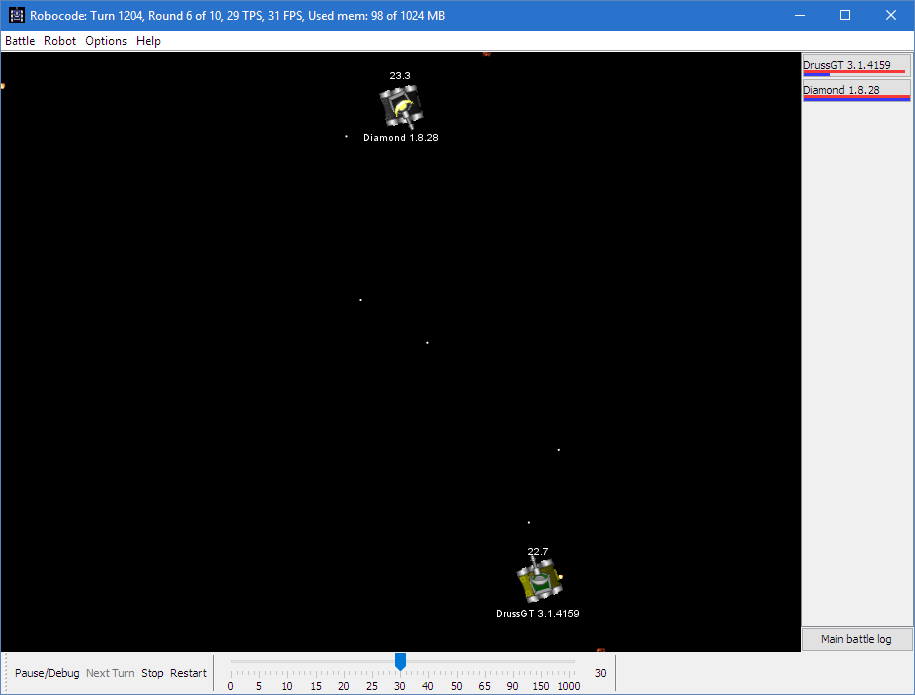
\includegraphics[width=0.80\textwidth]{figures/screenshot.png}
\caption{Screenshot from the Robocode battle arena. (Image credit: robowiki.net user MultiplyByZer0)}
\label{fig:screenshot}
\end{figure}

\textit{From http://robocode.sourceforge.net/docs/ReadMe.html}:
Robocode offers a complete development environment, and comes with its own installer, built-in robot editor and Java compiler. Robocode only pre-requires that a JVM (Java Virtual Machine) to exist already on the system where Robocode is going to be installed. Hence, everything a robot developer needs to get started is provided with the main Robocode distribution file (robocode-xxx-setup.jar). Robocode also supports developing robots using external IDEs like Eclipse.

Robocode is an Open Source project, which means that all sources are open to everybody. In addition, Robocode is provided under the terms of EPL (Eclipse Public License). The Robocode game was originally started by Mathew A. Nelson as a personal endeavor in late 2000 and became a professional one when he brought it to IBM in July 2001. In the beginning of 2005, Mathew convinced IBM to release Robocode as Open Source on SourceForge. Eventually, Flemming N. Larsen took over the Robocode project at SourceForge as administrator and developer in July 2006 to continue the original Robocode game -- which now is hosted on GitHub.

\section{Project overview}
Each project group will develop a robot using established software engineering practices. Furthermore, each group will compose a robot team to compete in a ``LU Rumble'' at the final lecture in the course. However, no project group is allowed to field their own robot -- instead robots developed by other groups must be purchased on an open market (in truth, a somewhat regulated market). Consequently, each project group has two primary goals: 1) maximizing profit by selling a successfully engineered robot on the market and 2) winning the LU Rumble by composing a competitive Robocode team. Project groups pursue the two goals by completing three main activities that we refer to as \textit{strategizing}, \textit{engineering}, and \textit{monetizing}, respectively.

Figure~\ref{fig:overview} shows the four main phases of the project. First, during the course inception, the course infrastructure and the project tasks are introduced. More importantly, project groups consisting of six students (preferably!) are established. Second, the backbone of the course follows: three development sprints mixing engineering, monetizing, and strategizing. Third, purchasers of robots perform acceptance testing to ensure that the delivered robot fulfills the expectations -- otherwise purchasers file business claims to require money back. Fourth, in the last phase of the project, the LU Rumble takes place followed by an awards ceremony to recognize the winning robot team -- and the most profitable project groups.

\begin{figure}
\centering
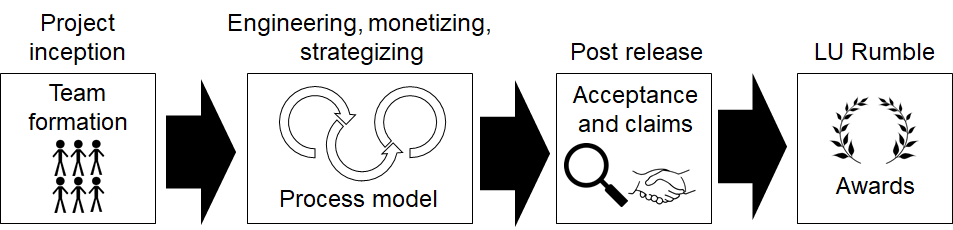
\includegraphics[width=0.99\textwidth]{figures/projectOverview.png}
\caption{The four phases of the project. Expect also a post mortem phase, concluding with the take-home exam.}
\label{fig:overview}
\end{figure}

Figure~\ref{fig:context} shows the context of each individual group during the project. Organizationally, your group has three divisions: 1) engineering, 2) purchasing, and 3) sales. Your group will assign the following roles: 1) project manager, 2) requirements engineer, 3) development lead, 4) test lead, 5) domain expert, and 6) sales engineer. Each role is described in detail in Section~\ref{sec:roles}.

Project groups do not exist in isolation, instead they act in a business ecosystem. During engineering of the robot, each project group will be part of two supplier-customer relationships. First, your sales engineer will be responsible for promoting sales of the robot under development. The domain expert of another project group will sign a contract of sale, establishing a formal relationship. Your sales engineer will be the primary communication point for the purchasing group's domain expert, i.e., a supplier-customer relationship involving feedback, feature requests, and negotiations. Second, analogously, your domain expert will act as the customer in a supplier-customer relationship with another project group. Note that, in some cases, project groups might buy from and sell to the same other group -- this is not regulated in the ecosystem.

On top of the two supplier-customer relationships, your project group will also communicate with the regulatory body (represented by your project supervisor). Your project group will hand in various signed contracts to the regulatory body, turn to it if to get support during supplier-customer negotiations, and to report the results from your acceptance testing. The regulatory body might also contact you with regulatory changes during the course of the project. Finally, you will practice one-way communication with the Robot Market, i.e., the open market where you will sell your Robot. All project groups will complement their robot teams with additional robots during the last week of the project -- and your sales engineer will be responsible for maximizing sales of your robot. 

\begin{figure}
\centering
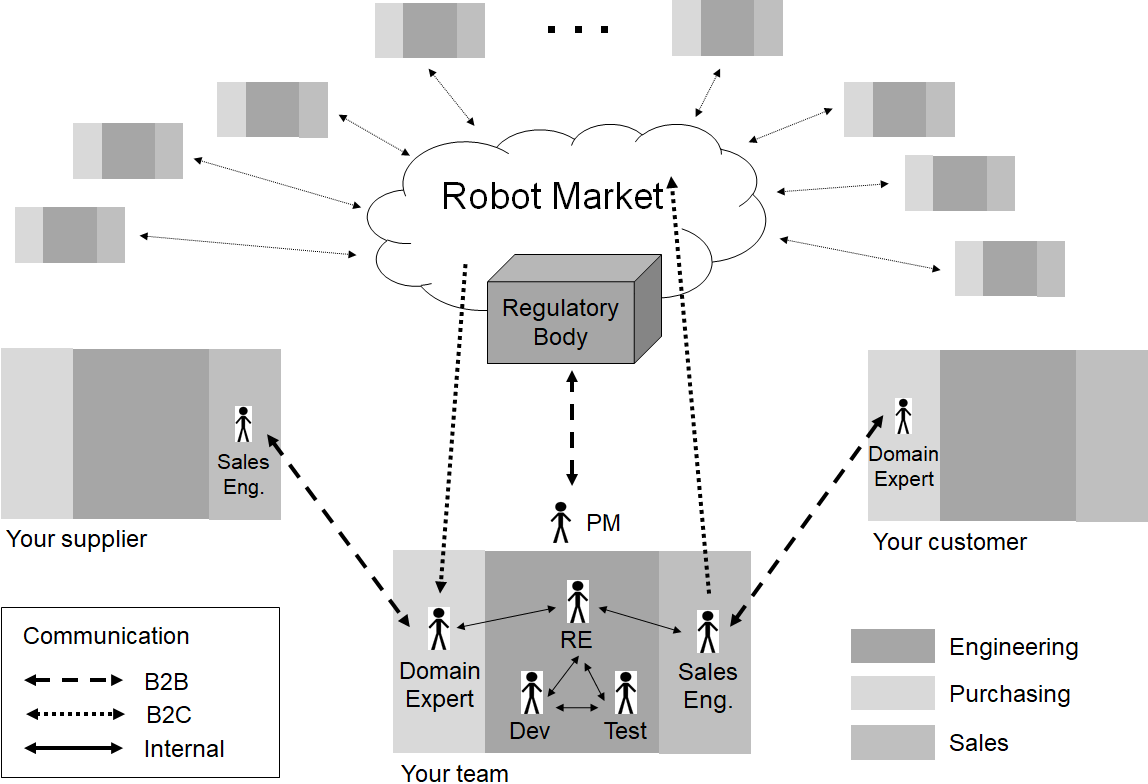
\includegraphics[width=0.99\textwidth]{figures/projectContext.png}
\caption{The project context. Your project group will interact with your supplier's sales engineer, your customer's domain expert, the open Robot Market, and the regulatory body.}
\label{fig:context}
\end{figure}

\section{Project grading}
\textit{To be written...}\\\\
The project will be graded as 3, 4, 5 or UG. TODO: Group grading and individual grades.

The project supervisors' overall grading guidelines include the following:
\begin{itemize}
\item The final release meets the final requirements specification. This is partly indicated by the customer's successful acceptance testing.
\item The delivered robot is successful and non-trivial.
\item All the robots behaviors are covered by the requirements specification.
\item The test specification describes a comprehensive verification of the robot. Automated test cases and test reports are provided.
\item The project group adhered to the process model and met all deadlines.
\item All deliverables are of high quality. Appropriate technical language and a consistent look-and-feel across documents.
\end{itemize}

\chapter{The project from a bird's eye view}
The project consists of three main activities, interconnected as presented in Figure~\ref{fig:components}. This section presents an overview of the three activities.

\begin{figure}
\centering
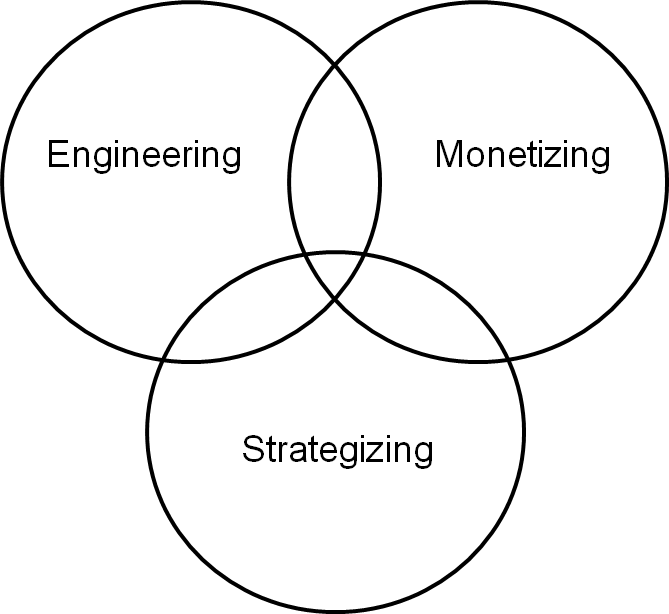
\includegraphics[width=0.40\textwidth]{figures/projectComponents.png}
\caption{Project components.}
\label{fig:components}
\end{figure}

\section{Engineering the robot}
Each project group will develop a robot (see Figure~\ref{fig:robot}) according to established engineering principles. These principles include product prototyping, integrated requirements engineering, and automated testing. The process model is organized in three development sprints, further described in Section~\ref{sec:process}. The engineering process is dominated by three core activities: \textit{specification}, \textit{construction}, and \textit{verification}. In line with agile development methodologies, all sprints consist of a mix of these three activities. Still, the groups' focus during the project will progress from specification, through construction, to verification -- also reflected by the order of the lectures.

\begin{figure}
\centering
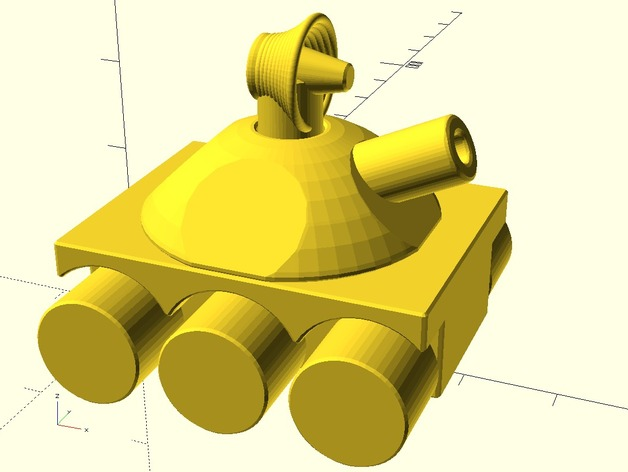
\includegraphics[width=0.50\textwidth]{figures/robotSide.jpg}
\caption{Model of the Robocode robot (\copyright~Klaus Knopper under CC BY-SA 3.0).}
\label{fig:robot}
\end{figure}

\subsection{Specification}
Requirements engineering, i.e., a systematic approach to developing a product with an end-user perspective, will be an integrated activity throughout the project. The requirements will be captured in a Software Requirements Specification (SRS) adhering to a template structure provided by the Institute of Electrical and Electronics Engineers (IEEE). IEEE is the world's largest technical professional organization, and a natural resource for software engineers -- possibly contented by the Association of Computing Machinery (ACM). Both organizations support engineers in development of software products adhering to state-of-practice approaches and provide ethical guidelines.

The IEEE SRS template provides a standard document structure: 1) an introduction section, 2) an overall description of the product under development, and 3) a list of product features further broken down into detailed requirements. Furthermore, the template supports engineers to specify quality requirements such as performance, maintainability, and memory footprint. Project groups are recommended to use a combination of traditional requirements of ``shall'' format and step-wise use case descriptions. While also user stories are covered in the lectures, it uses a narrative style that is less appropriate for development of autonomous robots.

The SRS connects all roles in the project group. While the requirements engineer is responsible for the SRS, the sales engineer is responsible for developing a sales pitch based on its content. The SRS will be public on the Robot Market, i.e., when other project groups consider purchasing your robot, they will critically review your SRS. The domain expert, having the most chance to predict what features will be valued on the Robot Market, will provide important input to the SRS -- effectively acting as a proxy-customer until the supplier-customer relationship has been established. Finally, the development lead is responsible for implementing the SRS in source code and the test lead is responsible for verifying that the developed product fulfills the SRS.

There are several quality attributes that a high-quality SRS should comply with. First, the SRS should be complete, i.e., if properly implemented, the developed product shall be a competitive robot. Just as importantly, the robot shall not offer any features that are not properly captured in the SRS -- the customer is not allowed any surprises. Second, the SRS should constitute a coherent document that is easy to follow. Furthermore, each individual requirement should be:

\begin{description}
\item[Complete] All information needed to implement source code to fulfill the requirement shall be specified. Developers must not be forced to read between the lines.
\item[Consistent] There are no contradictions between individual requirements.
\item[Feasible] The requirement can be practically implemented by the developers given the available resources. Also, the requirement will bring value to the end user or another stakeholder.
\item[Modifiable] An SRS is rarely static, thus all requirements must be able to change. Each requirement should be clearly identifiable.
\item[Unambiguous] A requirement shall only be interpretable in one way, i.e., no subjectivity can exist. Quality requirements should be quantified, not described using vague adjectives.
\item[Design free] Requirements shall specify what the system must or must not do, but not how the software will ensure the requirement is met -- leave that to the construction phase.
\item[Testable] Requirements shall be possible to verifiable, preferably by testing, otherwise inspection. 
\end{description}

As a result from the specification activities, each project group shall produce the following deliverables, further described in Section~\ref{sec:process}:
\begin{description}
\item[Sprint 1] SRS v0.5 -- Main features captured
\item[Sprint 2] SRS v0.9 -- Detailed requirements specified
\item[Sprint 3] SRS v1.0 -- A complete Robot specification
\end{description}

\subsection{Construction} \label{sec:constr}
The first two computer labs will help project groups set up Robocode development in Eclipse and source code control in git. Moreover, the second computer lab will initiate automated unit testing, an activity that overlaps construction and verification.

An early construction activity is software design. In this project, the design is limited to object-oriented design -- the robot development is too restricted to address any considerations on the software architecture level and there is also no user interaction design. Each project group will present the Object-Oriented Design (OOD) using a Unified Modeling Language (UML) class diagram. As the project in inspired by agile development methodologies, there will be no big design activity upfront. Instead, the OOD will evolve as the construction phase proceeds. The development lead is responsible to complement the final source code delivery with a class diagram to describe the OOD after-the-fact. Any project group that recognizes a value in using class diagrams in their robot sales pitch are of course welcome to do so. Furthermore, the final source code deliverable shall be complemented by Javadoc documentation.  

As most practical construction work will be done outside of scheduled sessions, how the backbone of the programming will be conducted must be decided by the individual project groups. Still, for this project, we recommend groups to follow a handful of well-known agile development practices, originally proposed as part of Extreme Programming (XP) [REF]. Below we list five that we believe are particularly suitable for the process model, along with their Wikipedia definitions:

\begin{description}
\item[Pair programming] All code is produced by two people programming  on one workstation. One programmer has control over the workstation and is thinking mostly about the coding in detail. The other programmer is more focused on the big picture, and is continually reviewing the code that is being produced by the first programmer. Programmers trade roles after minute to hour periods. The pairs are not fixed; programmers switch partners frequently, so that everyone knows what everyone is doing, and everybody remains familiar with the whole system, even the parts outside their skill set. This way, pair programming also can enhance team-wide communication and goes hand-in-hand with the concept of Collective Code Ownership.
\item[Continuous integration] The development team should always be working on the latest version of the software. Since different team members may have versions saved locally with various changes and improvements, they should try to upload their current version to the code repository every few hours, or when a significant break presents itself. Continuous integration will avoid delays later on in the project cycle, caused by integration problems, aka. ``big bang integration''.
\item[Code refactoring] Restructuring existing code without changing its external behavior. Refactoring improves quality attributes of the software, e.g., code readability, performance, maintainability. Refactoring is often initiated when a so called ``code smell'' is identified, i.e., structures in the code that indicate violation of fundamental design principles and negatively impact design quality. 
\item[Test-driven development] Create unit tests before the eventual code is written. This approach is intended to stimulate the programmer to think about conditions in which his or her code could fail. Test driven development proceeds by quickly cycling through the following steps: 1) write unit tests, 2) run tests, watch them fail, 3) write code, 4) run tests, watch them pass, and 5) refactor the code. Adhering to test-driven development leads to a large set of test cases that can be automatically executed, increasing developers' confidence when e.g. refactoring code.
\item[Collective code ownership] Everyone is responsible for all the code; therefore, everybody is allowed to change any part of the code. Collective code ownership is not only an organizational policy but also an attitude. Pair programming, especially overlapping pair rotation, contributes to this practice: by working in different pairs, programmers better understand the system context and contribute to more areas of the code base. Collective code ownership may accelerate development because a developer who spots an error can fix it immediately, which can reduce bugs overall. However, programmers may also introduce bugs when changing code that they do not understand well. Sufficiently well-defined unit tests should mitigate this problem: if unforeseen dependencies create errors, then when unit tests are run, they will show failures.
\end{description}

The construction phase involves prototyping to quickly create a working robot. Prototyping supports specification activities by enabling early executable software -- truly beneficial in contexts where the requirements are very unstable. Already at the end of sprint 1, around the LU Robot Fair, the project group shall deliver a first prototype of the robot. The prototype will help the purchaser to understand your product vision, and enable better feedback. The second deliverable shall be a Minimum Viable Product (MVP) inspired by lean software development practices [REF], i.e., a product with just enough features to satisfy early customers and to stimulate feedback for future robot evolution throughout Sprint 3. 

As a result from the construction activities, each project group shall produce the following deliverables. Each release shall be prepared as two jar-files: 1) one jar-file for customers and 2) one jar-file with embedded source code for the regulatory body. As previously stated, the final release to the regulatory body shall be complemented by a class diagram and Javadoc documentation, as further described in Section~\ref{sec:process}:
\begin{description}
\item[Sprint 1] Robot Alpha release (Robot v0.5) -- A prototype
\item[Sprint 2] Robot Beta release (Robot v0.9) -- An MVP
\item[Sprint 3] Robot Final release (Robot v1.0) -- The final robot
\end{description}

\subsection{Verification}
The first two computer exercises will introduce working with the JUnit framework for automated testing. Project groups will work with unit testing as a natural companion to the programming during development. While JUnit is designed for automated execution of unit test cases, groups will also use JUnit for system testing of both functional and non-functional (quality) aspects of the robot under development. Finally, groups will learn to use measure code coverage and use static code analysis tools to support software quality assurance.

The test lead is responsible for delivering three growing development artifacts during the projects, as well as a final test report at the final release. First, a suite of automated unit test cases shall evolve during the project. At sprint 1, an initial version shall simply be executable, but at the final release all source code shall be exercised by unit tests. Second, a suite of automated system test cases shall be developed -- an initial version at sprint 2, and the complete suite with the final release. Third, a Software Test Specification (STS) that describes the project group's test and quality activities. At sprint 3, all requirements in the SRS shall be verified either by automated test cases or targeted by a convincing argumentation that the requirement has been verified through inspection.

Verification activities are naturally supported by tools. Apart from the JUnit framework, the project groups will use Eclipse plugins to measure code coverage and a set of static analysis tools to automatically analyze the source code from different quality perspectives. TODO: describe the tools to use.

The final robot release shall be accompanied with a test report, signed by the test lead, showing that all test cases have been executed -- and all corresponding test verdicts. The customer will surely expect that all test cases passed, i.e., that you provide evidence that the entire SRS has been fulfilled by the final robot. In addition to the test verdicts, the test report shall contain appendices with extracted report from the code coverage tool as well as the static code analysis tools.

As a result from the verification activities, each project group shall produce the following deliverables, further described in Section~\ref{sec:process}:
\begin{description}
\item[Sprint 1] STS v0.5 -- Initial plan, especially regarding unit testing
\item[Sprint 2] STS v0.9 -- System testing specified
\item[Sprint 3] STS v1.0 and a signed test report
\end{description}

\subsection{Robot communication}
Your student group might want to implement communication between robots. To allow communication between robots developed by different suppliers, in practice creating a system-of-systems [REF], the ETSA02 Regulatory Body has standardized a communication protocol: ETSA02 RoboTalk. All messages transmitted between robots developed in the course should be transmitted as plain text strings, with one command per line. ETSA02 RoboTalk is version controlled, and groups that decide to implement communication should carefully specify in their SRS which version of the protocol is implemented.

ETSA02 RoboTalk will evolve during the course, i.e., the Regulatory Body will release new versions. All groups are welcome to provide feedback and requests to the standardization work done by the Regulatory Body. To do so, the project manager should submit a ``Change Request'' to the Regulatory Body. The Change Request should carefully describe what changes are proposed, and motivate why this request should be considered.

In short, robots that extend TeamRobot can communicate with their team members. If you want to implement this feature, please study the Robocode API:\\http://robocode.sourceforge.net/docs/robocode/robocode/TeamRobot.html\\Note that the MessageEvent always contains the name of the sending robot and a specific message.\\

Broadcasting message to all team members:
\begin{verbatim}
public void broadcastMessage(Serializable message)
\end{verbatim}

Sending messages to one specific team member:
\begin{verbatim}
TeamRobot.sendMessage(String name, Serializable message)
\end{verbatim}

When a robot receives a message, the following method is called:
\begin{verbatim}
onMessageReceived(MessageEvent)
\end{verbatim}

A message string should have the following overall structure, including the new lines.

\begin{verbatim}
[0-1] leadership;[followMe|leadMe]
[0-1] teamMode;[offensive|defensive]
[0-1] myPos;x;y
[0-*] friendPos;x;y
[0-*] enemyPos;x;y
[0-1] targetEnemy;name
[0-1] targetPos;x;y
[0-1] moveTo;x;y
\end{verbatim}

Example message:

\begin{verbatim}
teamMode;offensive
myPos;100;100
enemyPos;50;50
enemyPos;200;150
targetPos;50;50
\end{verbatim}

The commands shall have the following meaning:

\begin{description}
\item[leadership] Tells the receiving robot(s) that the sender takes on leadership (followMe) or reports as a follower (leadMe)
\item[teamMode] Tells the receiving robot(s) that the team shall enter offensive mode (offensive) or defensive mode (defensive)
\item[myPos] Tells the receiving robot(s) its current position on the 2D battlefield
\item[friendPos] Tells the receiving robot(s) the position of an identified robot in the same team
\item[enemyPos] Tells the receiving robot(s) the position of an identified enemy robot
\item[targetPos] Tells the receiving robot(s) to fire at a specific position on the 2D battlefield
\item[targetEnemy] Tells the receiving robot(s) to target a specific enemy robot
\item[moveTo] Tells the receiving robot(s) to move to a specific position on the 2D battlefield
\end{description}

\section{Monetizing the robot}
One of the primary goals of the project is to maximize the profit of the group, i.e., monetizing the robot. The business aspects of the project involves a combination of bespoke software engineering and software engineering for an open market. All project groups will offer their robot on a highly competitive market -- consisting of the other groups, each with a \euro 100 budget to invest in a robot team for the LU Rumble.

The project groups will market their Robot already at a robot fair already after Sprint 1. At this early point in time, only an Alpha release of the robot will be available and an initial version of the SRS -- still, the sales engineer is responsible for developing a convincing sales pitch. All groups will get the chance to pitch their robot through a two minute video at the robot fair, and also present it online on the Robot Market, complemented by the most recent SRS.

After the robot fair, all project groups will submit a ``purchase array'' to the regulatory body. The purchase array consists of one element per group, and each element should contain an integer representing how much your group is willing to pay for the corresponding robot. You are not allowed to make an offer for your own robot, and you are not allowed to offer less than \euro 10 for any other robot. The purchase array should be signed by the domain expert and delivered as a physical copy to the regulatory body through the mailbox in ``grå skåpet''.

Figure~\ref{fig:array} shows an example of purchase arrays submitted to the regulatory body. The purchase arrays are never disclosed, the regulatory body matches project groups into supplier-customer relationships. In the example, cells with bold text show winning bids. Group D, highlighted with a white row, was particularly interested in Robots E, F, and C -- but unfortunately, other project groups offered more. Group D instead got to buy Robot B for \euro 15. Note that the highest bid for a robot can be a tie, such as for Robot A and G. In the case of Robot A, no project group offered more than the minimum \euro 10, which resulted in a (possibly unexpected) bargain buy. 

\begin{figure}
\centering
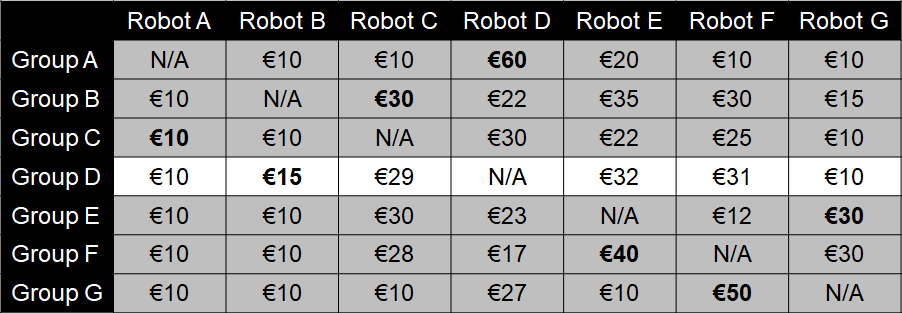
\includegraphics[width=0.80\textwidth]{figures/purchaseArray.png}
\caption{Example of seven purchase arrays submitted to the regulatory body.}
\label{fig:array}
\end{figure}

When all project groups have provided their purchase arrays, the regulatory body will commence its work to establish supplier-customer relationships. For each robot, the highest bidder turns into a customer of the group engineering the corresponding robot. If there is a tie, the customer relationship will be assigned randomly. In the end, all project groups will 1) pre-order a robot from a supplier, and 2) have a customer that offered at least \euro 10 to pre-order a robot (the price of the cheapest basic bot). Note that the decision of the regulatory body cannot be appealed. 

Once robots have been pre-ordered, 25\% of their costs will be transferred from the customer to the supplier. This amount will not be refunded in any case -- it represents the risks of purchasing a robot from an external organization. The remainder of the cost will be transferred at the delivery of the final robot. After the final delivery, the domain expert of the purchasing project group conducts acceptance testing of the robot. If the acceptance testing shows that delivered robot does not fully comply with the SRS, the project manager of the purchasing group is entitled to file a business claim to the regulatory body, further described in Section~\ref{sec:regbody}.

Each project group will also offer the robot under development on the Robot Market. After Sprint 3, all groups will seek to complement the pre-ordered (by now hopefully delivered) robot with additional robots to build a competitive robot team for the LU Rumble. Throughout Sprints 2 and 3, the sales engineer is responsible for promoting sales of the robot on Robot Market. Each group will also set a price for its robot -- a group must for at least ask as much as what the bespoke customer has paid. However, it is allowed for groups to offer discounts to buyers that purchase more than one robot, but the total cost must still be at least what the bespoke customer has paid. Note that this option is not available for suppliers of leader bots, as each team can field only one leader bot. Before the LU Rumble, the domain expert of each project group will sign purchase orders and deliver to the regulatory body through ``grå skåpet''. 

Figure~\ref{fig:market} shows an example of how two project groups purchase robots. After the robot fair, Group A strikes a deal with Group C. As Robot C was quite costly, Group A complements it with two cheaper droids from Robot B to create a robot team. On the other hand, Robot B resulted from bespoke development for Group C -- and they liked the result enough to buy two more at a later stage. Furthermore, Group C complements the cheap droids by two basic bots: a Basic Leader Bot and a Basic Bot. Both Groups A and C spend \euro95 of their budgets.

\begin{figure}
\centering
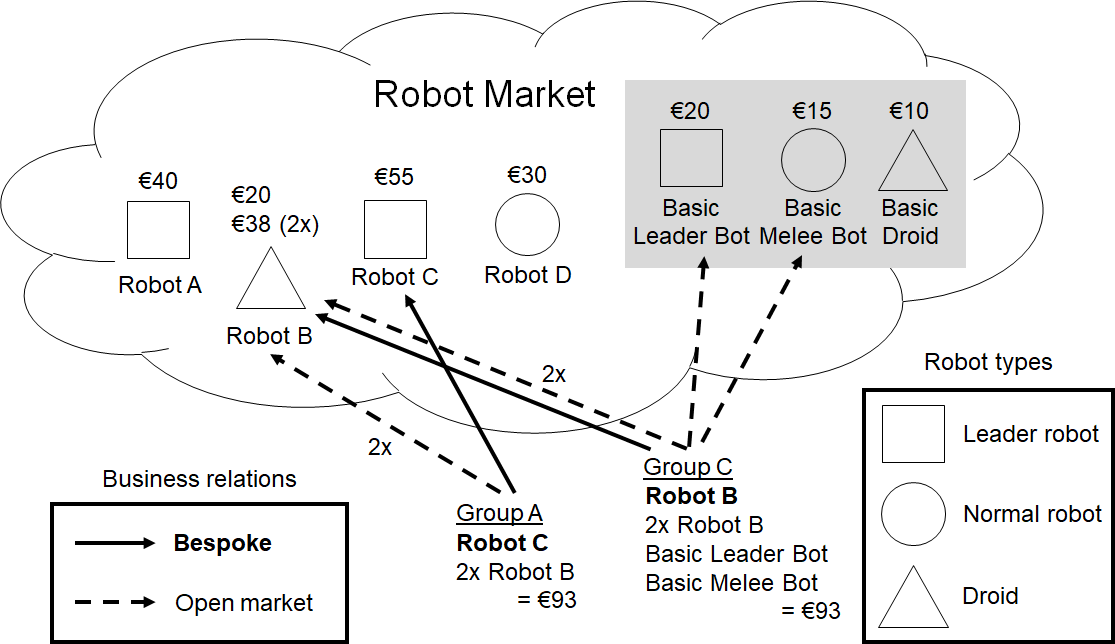
\includegraphics[width=0.85\textwidth]{figures/marketExample.png}
\caption{Example of two project groups purchasing robots for their teams.}
\label{fig:market}
\end{figure}

\section{Strategizing to win the LU Rumble}
The LU Rumble is a customized instance of a Robocode team rumble. Each project group will compose a team of up to five robots that will compete together against other robot teams. Each robot team must have one leader robot, which can be complemented by normal robots or droids.

As in any rumble, the goal is to reduce the energy of enemy robots to 0. Team robots will compete on a battlefield until only one team is left. A standard robot starts with 100 energy and is equipped with a radar and a gun turret. Each time the gun is fired, the robot loses energy according to the payload. If the bullet does not hit any target, the energy is lost. If the bullet hits another robot, energy is transferred from the hit robot to the firing robot.

Apart from the standard robots, there are two special types of robots. The leader robot has an additional 100 energy compared the normal robot. Droids have an additional 20 energy, but are not equipped with radars.

At the end of Sprint 1, your project group will have established a relationship with a robot supplier by pre-ordering either a leader robot, a normal robot, or a droid. The supplier will provide you with a final robot at the end of Sprint 3, but your group will have a chance to influence the evolution of the robot during Sprints 2 and 3. The domain expert in your group is responsible for developing a strategy around the robot you have pre-ordered -- to guide your feedback, you will receive two prototypes for evaluation: an Alpha release after Sprint 1, and a Beta release after Sprint 2.

At the end of Sprint 3, you will complement the robot you have ordered with other robots from the Robot Market. The goal of your strategizing is to identify and purchase additional robots that can successfully cooperate with the robot from your supplier. It is important to keep an eye on the Robot Market during Sprints 2 and 3, both to find the best robots to purchase, and to understand what type of features you should provide through your own robot under development. Note that three robots are always available at fixed prices: 1) BasicLeaderBot \euro 20, 2) BasicBot \euro 15, and 3) BasicDroid \euro 10.

Each robot team must adhere to two strict constraints: 

\begin{enumerate}
\item Each team must consist of between one and five robots, including one leader robot.
\item Each team must not exceed a total cost of more than \euro 100 worth of robots.
%\item The final team must be submitted as a jar-file to the LU Rumble on Friday morning before the event. 
\end{enumerate}

\chapter{Project phases}

\section{Project inception}
The first week of the project is referred to as the project inception. The project inception phase is dominated by project group development, i.e., forming groups, assigning roles, and aligning goals and expectations.

According to a well-known model of group development, proposed by Tuckman in 1965 [REF], four distinct phases are all necessary and inevitable for a group of people to face up to challenges, collaborate successfully, and to  deliver results. Being aware of the four phases might accelerate the less productive phases and mitigate group conflicts:
\begin{description}
\item[1. Forming] The group meets and learns about the project and the required activities. In the beginning, individuals tend to behave quite independently -- all trying to comprehend what is about to happen. Individuals might be motivated and on their best behavior, but typically the understanding and expectations vary considerably. 

In the project, groups will be established already during the break in the first lecture, i.e., before lunch the very first Monday. The individual group members are expected to read the project instructions carefully as early as possible.
\item[2. Storming] After a while, some disagreements and personality clashes are likely to emerge within the group. People are people, and people are different. Tolerance of each group member should be emphasized, otherwise the group will fail or rely on individual ``hero efforts''. This phase can become destructive to the group, and some teams will never develop past this stage. On the other hand, settling disagreements within the team can make members stronger, more versatile, and able to work more effectively together. Note that some groups never enter this stage at all, i.e., transitions directly from forming to norming are possible.

In the project, the supervisors and the regulatory body will be particularly responsive to questions and clarifications during the first week. Also, the group communication will be kick-started by two physical meetings soon after the formation, i.e., exercise sessions on Wednesday and Thursday the first week.

\item[3. Norming] Resolved disagreements and personality clashes lead to a spirit of co-operation -- this typically happens when the group becomes aware of the external competition and share a common goal. In this stage, all group members take the responsibility and agree to work for the success of the common goal. The group members accept others as they are and make an effort to move on. 

In the project, the first week concludes with assigning roles within the group, see Section~\ref{sec:roles}. All members of the group will also sign a collaboration contract, specifying the roles, and the intentions to collaborate successfully. The contract will be submitted to the regulatory body through ``grå skåpet''.
\item[4. Performing] When the group norms and roles have been established, focus is shifted to achieving common goals. However, groups might revert to earlier circumstances in certain circumstances, e.g., unexpected events, emerging personal conflicts, or changing leadership. In the project, the goal is of course to remain in the performing stage until the LU Rumble!
\end{description}

\section{Process model} \label{sec:process}
The process model describing the product development encompasses three sprints, each with a separate set of deliverables. 

\begin{figure}
\centering
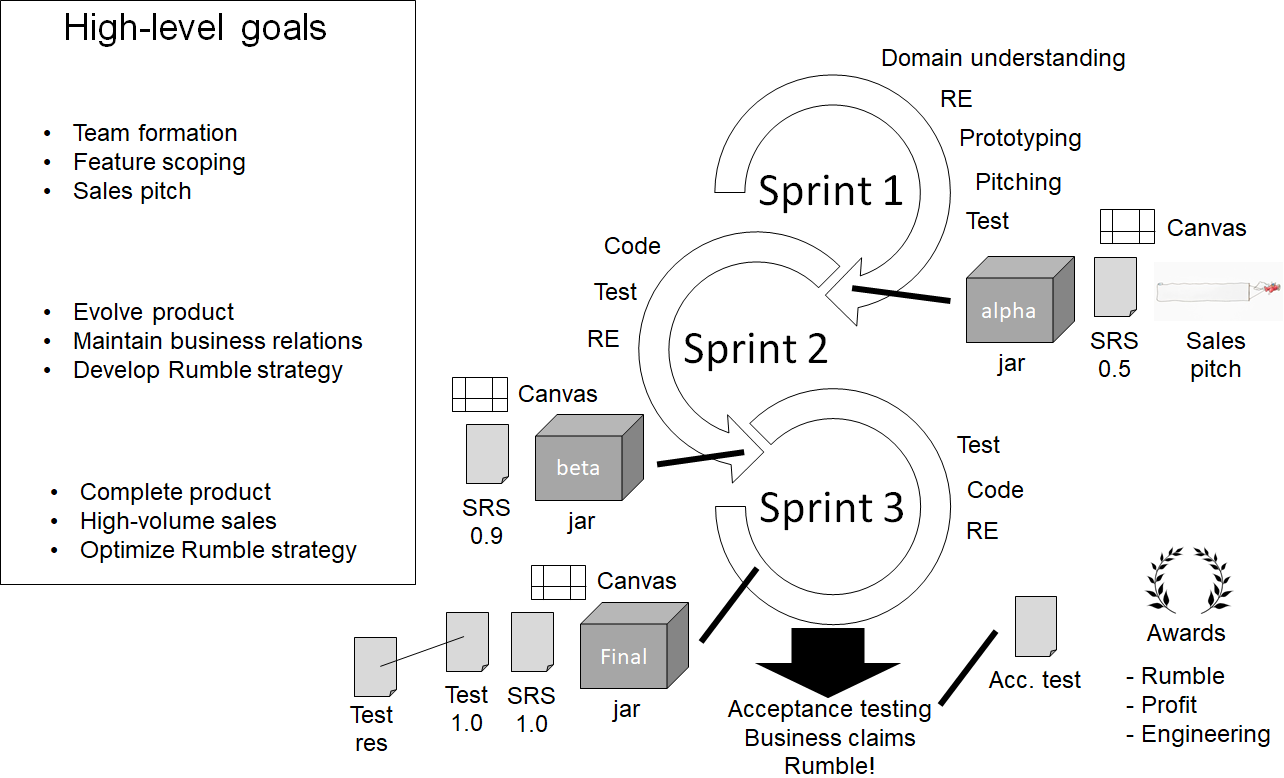
\includegraphics[width=1.0\textwidth]{figures/processModel.png}
\caption{The ETSA02 process model, organized in three sprints.}
\label{fig:overview}
\end{figure}

\subsection{Sprint 1}
The first sprint overlaps with the project inception as the groups will start working on robot development already at the first exercise sessions in the first week. The high-level goals of Sprint 1 are to successfully do: 1) feature scoping, 2) robot prototyping, and 3) developing a sales pitch. This means that the project group will be focused on engineering and monetizing during Sprint 1. Some strategizing will also occur, as the domain expert will purchase a robot from a supplier after the Robot Fair.

The first steps of the requirements engineering involves analyzing what type of robot would be in high demand by the other project groups. This type of market analysis is no easy task to conduct, and surely the requirements engineer will discuss intensively with the domain expert and the sales engineer. Engineering a software product means making a series of successful technology and business decisions, and already during Sprint 1 the project group needs to set the direction for the engineering department. High-level requirements are referred to as features, and the task of deciding which features to implement in the product is called \textbf{feature scoping}. At the end of Sprint 1, SRS v0.5 should specify the features the group intends to implement in their robot. The features should be promising enough to generate good offers by other project groups, but do not promise too much (aka. ``over scoping'') -- if you do not deliver a robot that fulfils the specification in the final release, your customer will most likely file business claims to the regulatory body! On the other hand, the SRS v0.5 is not carved in stone. There will be negotiations during Sprints 2 and 3, and if both the customer and the regulatory body accept your change requests, you can both modify and remove features later -- and adding new features is of course always possible.

A central part of the engineering in Sprint 1 is the \textbf{robot prototyping}, an activity that serves two main purposes. First, it helps your project group experiment with different candidate features for the robot under development. There is no better way to learn the Robocode domain than by practically implementing different approaches and evaluating them. Second, the prototyping will lead to an Alpha version of the Robot. The customer will obtain the Alpha release, which will enable much richer feedback than an SRS alone. To ensure that testing is part of the development process from the start, Sprint 1 will introduce unit testing in the second week.

The marketing concept is the strategy that an organization implements to satisfy customers needs, increase sales, maximize profit, and beat the competition. The customers' focus and values are the routes to achieve sales and maximize profits. In the project, the marketing concept is a customer-centered ``sense and responds'' philosophy. Your project group's job is not to find the right customers for your robot, but rather to find the right robot for your customers -- first for the long-lasting supplier-customer relationship, and later through the Robot Market. At the end of Sprint 1, the course will organize a Robot Fair. Each group will get a 2 minute slot to \textbf{pitch} their product through a video. All project groups will also have a folder to showcase promotion material on a ``Display window'' Google Drive folder shared with all groups.

Sprint 1 shall result in the following deliverables to the following stakeholders. The responsible role is shown in parentheses.

\begin{table}[]
\centering
\caption{Deliverables due after Sprint 1.}
\label{tab:sprint1}
\begin{tabular}{|p{4cm}|p{2cm}|p{2.5cm}|p{4.5cm}|}
\hline
\textbf{Deliverable}           & \textbf{Receiver}   & \textbf{Responsible role} & \textbf{When?}     \\ \hline
Lean canvas (latest version)   & Supervisor          & Project manager           & L3: Apr 16 - 12.00 \\ \hline
SRS v0.5                       & Customer+ Supervisor & Requirements engineer     & L3: Apr 16 - 12.00 \\ \hline
Robot Alpha version            & Customer+ Supervisor & Development lead          & L3:Apr 16 - 12.00  \\ \hline
STS v0.5        			   & Customer+ Supervisor & Test lead                 & L3:Apr 16 - 12.00  \\ \hline
Sales pitch + promotion folder & Course responsible  & Sales engineer            & L2: Apr 12 - 23.59 \textbf{(before Robot Fair!)}\\ \hline
Purchase array                 & ``Grå skåpet''      & Domain expert             & L4: Apr 17 - 23.59 \textbf{(after Robot Fair!)} \\ \hline
\end{tabular}
\end{table}

\newpage

To support Sprint 1, the following sessions are scheduled:
\begin{itemize}
\item Lecture 1: Robocode, Requirements engineering
\item Lab 1: Robot development in Eclipse
\item Exercise 1: Product planning
\item Lecture 2: Unit testing, git, object-oriented design
\item Lab 2: Refactoring and JUnit
\item Exercise 2: Marketing communications
\end{itemize}

\subsection{Sprint 2}
In Sprint 2, the project group should be up to speed both regarding engineering and monetizing. Now the monetizing will decrease and the strategizing will increase in its place. The high-level goals of Sprint 2 is to: 1) evolve the robot, 2) maintain the customer relationship, and 3) develop a strategy for the LU Rumble.

In Sprint 2, you will have an established customer who has received your Robot Alpha release. As that project group will be keen to win the LU Rumble, you will likely get feedback that they believe will guide your development to a successful robot. During the remainder of the project, maintaining a healthy \textbf{customer relationship} is critical. Your sales engineer is the main point of contact with the customer.

Based on your customer's feedback, your own vision -- and possibly some negotiation in between -- you will \textbf{evolve the robot} during Sprint 2. The features will be broken down into detailed requirements, and the STS will be elaborated to also cover system testing. At the end of Sprint 2, you will deliver Robot Beta release to your customer, constituting an MVP, i.e., a minimal product that still brings some value. To be in a good position for the next sprint, the project group should try to let the lean canvas, SRS, source code, STS, and marketing concept co-evolve -- otherwise they might diverge considerably, increasing the risk of a dissatisfied customer, wasted effort within your group, and reduced sales on the Robot Market. Make sure that any changes you make to the SRS are traceable, i.e., make sure there is a ``paper trail'', in case the regulatory body needs to settle business claims from your customer at a later stage. Significant changes to the SRS must be done in agreement with the customer and documented. If the supplier organization does not store a chain of evidence, the regulatory body is likely to side with the customer in legal contentions.

Finally, you will develop a first draft of your \textbf{Rumble strategy}. The cornerstone of your robot team will be the robot you pre-ordered. Your domain expert will be responsible for communication with your supplier's sales engineer. Just like your project group should be responsive to your customer, your supplier should respond to your requests.

Sprint 2 shall result in the following deliverables to the following stakeholders. The responsible role is shown in parentheses.
\begin{itemize}
\item The latest version of the lean canvas (Project manager)
\item SRS v0.9 to the customer and the regulatory body (Requirements engineer)
\item Robot Beta release to the customer (Development lead)
\item STS v0.9 to the regulatory body (Test lead)
\end{itemize}

To support Sprint 2, the following sessions are scheduled:
\begin{itemize}
\item Lecture 3:
\item 
\item
\end{itemize}

\subsection{Sprint 3}
In Sprint 3, the project group shall conclude and tie up all activities. The engineering should lead to a successful robot, the monetizing should ensure that it is well-received on the market, and the strategizing shall finalize the robot team shall be competitive in the upcoming LU Rumble. The high-level goals of Sprint 3 are to: 1) complete the product, 2) generate high-volume sales, and to 3) optimize the Rumble strategy.

The engineering department will be busy implementing the remaining requirements and putting the finishing touches to the robot. This means \textbf{completing the product} and preparing the Robot Final release. When the Final Robot is released, it is important that the lean canvas, SRS, STS, and the marketing concept are all aligned. Your customer will perform acceptance testing of your robot -- rest assured that they will scrutinize your deliverables to identify any discrepancies. The customer will be greatly motivated to assure that the Robot Final release complies with the SRS -- their entire robot team for the LU Rumble might rely on it! If the customer is not satisfied, the regulatory body is likely to receive a business claim based on their acceptance testing. However, your project group will provide the regulatory body with evidence that everything in the SRS has been verified by providing a complete test report based on STS v1.0.
 
The sales department will keep active communications with the customer, to make sure the final engineering efforts adhere to their expectations. Close communication with the customer will reduce the risks of incoming business claims. However, the sales engineer will also focus considerable effort on the robot offering on Robot Market -- trying to make the robot as attractive as possible on the open market, i.e., the sales engineer will maintain the Robot webpage with the intention to \textbf{generate high-volume sales}.

The purchasing department will keep a close eye on the engineering efforts of the supplier. After all, this is the supplier's last chance to deliver the robot that has been specified in the SRS. At the same time, your domain expert will analyze the Robot Market to make a final decision of your robot team composition, i.e., \textbf{optimizing the Rumble strategy}. 

Sprint 3 shall result in the following deliverables to the following stakeholders. The responsible role is shown in parentheses.
\begin{itemize}
\item SRS v1.0 to the customer and the regulatory body (Requirements engineer)
\item Robot Final release to the customer and the regulatory body (Development lead)
\item STS v1.0 to the regulatory body and the customer (Test lead)
\item Test report to the regulatory body and the customer (Test lead)
\item A robot team composition to the regulatory body (Domain expert)
\end{itemize}

To support Sprint 3, the following sessions are scheduled:
\begin{itemize}
\item Lecture 4:
\item 
\item 
\end{itemize}

\section{Post release}
The phase following the process model is referred to as post mortem. In this phase, your project group will perform acceptance testing of your supplier's Robot Final release. If the acceptance testing identifies flaws, you will file business claims to the regulatory body -- possibly deducting from the total payment. Furthermore, after settling the business claims, the domain expert will submit the final purchase orders to the regulatory body, i.e., the robot team composition for the LU Rumble will be finalized.

The post mortem shall result in the following deliverables to the following stakeholders. The responsible role is shown in parentheses.
\begin{itemize}
\item Acceptance test report (Domain expert)
\item (Potentially) Business claims (Project manager)
\item Purchase orders to the regulatory body (Domain expert)
\item A robot team composition to the regulatory body (Domain expert)
\end{itemize}

\section{LU Rumble}
The final phase consists of one single event: the LU Rumble. The LU Rumble will take place during the final lecture of the course on May 21, 2018.

Prior to the event, the regulatory body will run a qualification session, inspired by the format used in Formula one racing. The purpose of the qualification session is twofold. First, it assures that all robot teams are functional on the Robocode arena. Second, it will let a number of robot teams get ``pole positions'', i.e., seeds for the LU Rumble main tournament. The qualification session entails a large number of simulations between all teams. Note that while the qualification session will indicate some robot teams as favourites, they might be good on average, but have weaknesses against certain team strategies. No matter the results of the qualification session, all robot teams can still win the LU Rumble.  

The main tournament, i.e., the playoff, will follow a cup pairing according to single elimination knockout rules. The four robot teams performing the best during the qualification session will be seeded into the tournament bracket. All remaining robot teams will enter the bracket at random. Each match in the LU Rumble will be played in best-of-five format, and displayed live at reasonable speed for the entertainment of the spectators.

Immediately after the LU Rumble, three awards will be given:
\begin{itemize}
\item The Strategizer Award goes to the winner of the LU Rumble.
\item The Monetizer Award goes to the most profitable project group.
\item The Engineering Award is a people's choice with voting during the LU Rumble (or a jury in the regulatory body?).
\end{itemize}

\chapter{Inter-group communication}
\emph{To be written...}\\\\

\section{The regulatory body} \label{sec:regbody}
\emph{To be written...}\\\\
Formal document templates:

\begin{itemize}
\item Contract of sale between supplier and customer
\item Purchase order for Robot Market
\item Business claims
\end{itemize}

\section{Maintaining supplier-customer relations}
\emph{To be written...}\\\\
What to do and what not to...\\

Guidelines for suppliers:
\begin{itemize}
\item The customer is always right
\item Do not sacrifice the chance to succeed on the open market
\item Be open to new ideas from the customer.
\item Embrace change -- it is inevitable anyway.
\item Negotiate nicely.
\end{itemize}

Guidelines for customers:
\begin{itemize}
\item Accept what you've pre-booked.
\item Do not provide feedback that deviates from the original vision of the robot.
\item Be open to alternative solutions proposed by the supplier.
\item Negotiate nicely.
\end{itemize}

\section{Group conflicts}
\emph{To be written...}\\\\

\chapter{Detailed instructions}
This section presents some aspects of the course in detail: 1) the roles you should assign within the project group, 2) expectations on the deliverables, and 3) the course infrastructure.

\section{Role assignment} \label{sec:roles}
During the course, all students are expected to contribute to all activities. The purpose of the roles is not to isolate work tasks that could be individually completed. Software engineering is a collaborative effort, and completing work tasks in isolation is not part of a scalable methodology. Instead, we stress the value of ``collective ownership'' during the project, not only for the source code as described in Section~\ref{sec:constr}, but for all artifacts produced.

The purpose of assigning roles in the project is to comply with the ETSA02 course description regarding ``judgment and approach'', i.e., understanding that software engineering is a complex endeavor involving several different roles, and that working as a software engineer might  result in a variety of roles in an organization. Second, all roles with be responsible for some deliverables. The regulatory body will use the group member with the corresponding role as the primary point of contact in case any deliverable is missing or critically incomplete.

As the project progresses through phases and sprints, different roles with have different expectations. The project group will track the variation through weekly time reporting, submitted by the project manager to the regulatory body. The reported figures should be complemented by a qualitative analysis of the causes, and the project manager is responsible for balancing the workload to make sure the contributions are comparable, see~\ref{sec:time} for further information. Below are the different roles, ordered alphabetically:

\begin{description}
\item[Development lead] Design, implementation, source code quality. Assign a group member comfortable with the art and science of programming. -- jar_v0.5, jar_v0.9, jar_v1.0
\item[Domain expert] Mastering Robocode, LU Rumble strategy, supplier communication, negotiations, acceptance testing. The domain expert needs to be willing to learn about the game aspects of Robocode, thus pick your gamer. -- Signed contract (as customer), acceptance test report, team jar-file
\item[Project manager] Coordination, time reporting, communication with the regulatory body. Identify a group member with leadership skills willing to shoulder overall responsibilities. -- Weekly time reports with reflections, business claims (based on failed acceptance test)
\item[Requirements engineer] End-user perspective, feature scoping, detailed requirements. A requirements engineer bridges engineering and business, identify a generalist. -- SRS v0.5, SRS v0.9, SRS v1.0
\item[Sales engineer] Marketing, sales pitch, customer communication, negotiations. Identify your natural salesman, a person with excellent communication skills. -- Sales pitch, signed contract (as supplier)
\item[Test lead] Test strategy, unit testing, system testing. Suitable for an individual with an eye for details. -- Unit tests, STS v1.0 (incl. test code), test results
\end{description}

\section{Time reporting and reflections} \label{sec:time}
\emph{To be written...}\\\\
Report time per role on a weekly basis. Reflect on the figures after each sprint. Plan changes if needed to better balance the work load.

\section{Software Releases: Alpha, Beta, and Final}
The robot shall be released after each development sprint, each time constituting a more mature software product. In ETSA02, you shall create each software release in two variants: 1) a customer release and 2) a regulatory body release. Groups will upload their releases in designated folders on Google Drive.

The customer release shall contain the latest versions of the following:

\begin{itemize}
\item SRS
\item Robot packaged as a jar-file -- without source code!
\item STS
\item Optional: Release notes -- if you want to clarify anything related to the release. Simply create a text file called ``ReleaseNotes_vX.txt'' and replace X with 0.5, 0.9, or 1.0.
\end{itemize}

The regulatory body release shall contain everything in the customer release, but also the latest version of the following artifacts:
\begin{itemize}
\item Lean canvas
\item Robot packages as a jar-file -- including source files!
\item Class diagram
\item Javadoc
\end{itemize}

\chapter{Expectations per deliverable}
This section briefly explains what is expected of the various deliverables.

\begin{description}
\item[Collaboration contract] The first deliverable is a contract signed by all group members, stating agreed upon collaboration rules and the role assignment within the group.
\item[Sales pitch] A video pitch to be played at the Robot Fair, not longer than 2 min. The video shall be recorded in a standard video format, but you are free to choose the structure and content. For example, you can choose whether to record yourself speaking, a screencast, or a mix of both. The sales pitch shall communicate your message, you are not supposed to complementing it during the Robot Fair with live talking. You are of course no allowed to include any offensive or illegal content in the marketing communications. You will also get a shared folder on Google Drive which you can use freely to promote your sales -- be creative!
\item[SRS] The software requirements specification shall be delivered in three versions. Each version should be a more mature specification of the robot under development.
\begin{description}
\item[v0.5] A skeleton of an SRS adhering to the provided template. The main features that will be implemented shall be listed.
\item[v0.9] The features shall be broken down into detailed requirements.
\item[v1.0] A final SRS that provides a complete specification of the robot.
\end{description}
\item[The robot] The robot shall be released in three versions: Alpha, Beta, and Final. The lead developer shall each time package the robot as jar-files using the Robot Packager in Robocode, in two different versions per release: 1) without source files for the customer, and 2) including source files for the supervisor. The source code shall be maintainable, e.g., well-structured, commented, and using suitable variable names.
\begin{description}
\item[Alpha] An early prototype of the robot. No expectations regarding features, but the customer shall be able to field it in a Robocode battle.
\item[Beta] TBD
\item[Final] TBD
\end{description}
\item[Class diagram] The object-oriented design shall be documented in a UML class diagram. You can use any tool to create the diagram, either a tailored UML tool or a standard drawing tool -- you can even scan a pen and paper sketch or take a picture of a whiteboard drawing.
\item[Javadoc] The robot source code shall be documented and packaged using the standard Javadoc tool.
\item[STS] The document shall describe how the group uses testing to increase the quality of the robot, i.e., what measures are taken to decrease the risk of releasing a product with bugs. Furthermore, system test cases used to verify that the SRS is completed shall be specified.
\begin{description}
\item[v0.5] A first draft of an STS adhering to the provided template.
\item[v0.9] TBD.
\item[v1.0] TBD.
\end{description}
\item[Test report] The final release shall be accompanied by a test report that shows that all system test cases have been executed. Each system test case shall be listed, and you shall report the date when it was executed and its result.
\item[Purchase array] The purchase array shall specify valid offers for all other groups robots and be signed by the domain expert.
\item[Acceptance test report] When the final release of another group's robot has been received, you shall test it to see if it complies with its SRS. You shall write an acceptance test report clearly stating how you tested the robot and what the results were. You are free to choose a format for the document.
\item[Business claims] This is an optional deliverable that you can send to the regulatory body. If you are not satisfied with the final release you received from another group, you can argue for your case in a written business claim. You are free to choose a format for the document. 
\end{description}

\section{Project infrastructure}
\emph{To be written...}\\\\
The following infrastructure is central during the project:

\begin{description}
\item[SRS template]
\item[Slack workspace]
\item[Contract templates]
\item[Collaboration contract]
\item[Contract of sales]
\item[Time reporting]
\item[Robot team composition sheet]
\end{description}

\end{document}
